\documentclass[review]{elsarticle}

\usepackage{lineno,hyperref}
%\modulolinenumbers[5]
\usepackage{amsmath,amssymb,amsfonts}
\usepackage{algorithm,algorithmic}
\usepackage{graphicx}
\usepackage{makecell}
\usepackage{textcomp}
\usepackage{xcolor}


\journal{Applied Energy}

%%%%%%%%%%%%%%%%%%%%%%%
%% Elsevier bibliography styles
%%%%%%%%%%%%%%%%%%%%%%%
%% To change the style, put a % in front of the second line of the current style and
%% remove the % from the second line of the style you would like to use.
%%%%%%%%%%%%%%%%%%%%%%%

%% Numbered
%\bibliographystyle{model1-num-names}

%% Numbered without titles
%\bibliographystyle{model1a-num-names}

%% Harvard
%\bibliographystyle{model2-names.bst}\biboptions{authoryear}

%% Vancouver numbered
%\usepackage{numcompress}\bibliographystyle{model3-num-names}

%% Vancouver name/year
%\usepackage{numcompress}\bibliographystyle{model4-names}\biboptions{authoryear}

%% APA style
%\bibliographystyle{model5-names}\biboptions{authoryear}

%% AMA style
%\usepackage{numcompress}\bibliographystyle{model6-num-names}

%% `Elsevier LaTeX' style
\bibliographystyle{elsarticle-num}
%%%%%%%%%%%%%%%%%%%%%%%

\begin{document}

\begin{frontmatter}

%\title{Innovative techno-economic optimization of stand-alone solar photovoltaic systems using automated formal synthesis} 
\title{An automated formal synthesis optimization method for sizing of stand-alone solar photovoltaic systems: case studies and comparative}
%
%\title{Elsevier \LaTeX\ template\tnoteref{mytitlenote}}
%\tnotetext[mytitlenote]{Fully documented templates are available in the elsarticle package on \href{http://www.ctan.org/tex-archive/macros/latex/contrib/elsarticle}{CTAN}.}
%
%% Group authors per affiliation:
\author[mymainaddress]{Alessandro Trindade\corref{mycorrespondingauthor}}
\cortext[mycorrespondingauthor]{Corresponding author}
\ead{alessandrotrindade@ufam.edu.br}
%\ead[url]{www.elsevier.com}

\author[mysecondaryaddress]{Lucas Cordeiro}


\address[mymainaddress]{Federal University of Amazonas, Av. Rodrigo Octávio, 6200, Coroado I, 69077-000 Manaus-AM-Brazil}
\address[mysecondaryaddress]{University of Manchester, School of Computer Science, Kilburn Building, Manchester M13 9PL}

\begin{abstract}
There exist various methods and tools to size solar photovoltaic systems; however, these existing tools are mainly based on simulations, which do not cover all aspects of the design-space during the search for the optimal solution. \textcolor{red}{Here, we present a novel sound and automated approach to obtain optimal sizing of stand-alone PV systems using program synthesis, with a particular focus on computer optimization methods instead of criteria or objectives, which were investigated in prior studies over the last two decades}. In particular, our variant of counterexample guided inductive synthesis (CEGIS) approach has two phases: first we synthesize the sizing of stand-alone PV systems based on power reliability, but that may not achieve the lowest cost; second, the proposed solution is then verified iteratively with a lower bound \textcolor{red}{cost} via symbolic model checking. If the verification step does not fail, the lower bound is adjusted; and if it fails, a counterexample is provided with the optimal sizing, thereby linking the technical response of the first phase with cost analysis of the second phase. Commercial equipment data from different manufacturers are provided to our synthesis engine and candidate solutions are derived from financial analysis of the obtained sizing. Our synthesis method is novel and unprecedented to streamline the design of PV systems. Experimental results using seven case studies show that our synthesis method is able to produce within an acceptable run-time the optimal PV system sizing. \textcolor{red}{We also present a comparative with a specialized simulation tool over real PV systems to show the effectiveness of our approach, which is able to provide more accurate results of optimal sizing of stand-alone PV systems than that existing simulation tool}.
\end{abstract}

\begin{keyword}
automated verification \sep model checking \sep program synthesis \sep electrical systems \sep solar photovoltaic systems
\end{keyword}

\end{frontmatter}

%\linenumbers

%%%%%%%%%%%%%%%%%%%%%%%%%%%%%%%%%%%%%%%%%%%%%%%%%%%%%%%%
\section{INTRODUCTION}
%%%%%%%%%%%%%%%%%%%%%%%%%%%%%%%%%%%%%%%%%%%%%%%%%%%%%%%%
Cyber-Physical Systems (CPS) are engineered systems, which are built from, and depend upon, the seamless integration of computational and physical  components~\cite{NSF2015}. During operation, such components must frequently adapt to the operating environment changes faced at run-time (dynamics of the physical processes) and must be able to continue to behave in a controlled and safe way, thus posing novel technical challenges for the software engineering of services and applications for CPS~\cite{Metzger2014}. Software pervasiveness in CPS places new challenges; in particular, highly dynamic environments, rapidly changing requirements, unpredictable and uncertain operating conditions demand new paradigms for software design~\cite{Filieri2015}.

While some research efforts do exist to enhance and optimize the software development processes for CPS, further investigation and discussion of better and more effective models are still needed in practice~\cite{Al-Jaroodi2016}. Among the opportunities for enhancements in the software development processes for CPS, there exists the need for developing new techniques and tools to support CPS requirements gathering and analysis with the goal of synthesizing \textit{correct-by-construction} implementations of CPS. These techniques need to deal with predefined requirements enforced by the nature and inherited constraints of the target CPS. In addition, they should be able to provide verification and validation mechanisms for completeness, correctness, and consistency~\cite{Al-Jaroodi2016}. Uncertainty and variability, at the same time, can be dealt with formal verification~\cite{NESSI}. Energy production, distribution, and optimization are all CPS problems~\cite{UC}. 

Lack of access to clean and affordable energy is considered a core dimension of poverty~\cite{Hussein2012}. Progress has been made worldwide; in particular, the number of people without electricity access fell below $1$ billion threshold for the first time in $2017$~\cite{IEAweo2018}. In order to provide universal electricity for all, decentralized systems led by solar photovoltaic (PV) in off-grid and mini-grid systems will be the lowest-cost solution for three-quarters of the additional connections needed~\cite{Hussein2012}; specifically grid extension will be the standard in urban areas~\cite{IEAweo2018}.

In order to simulate or evaluate a PV system, there exist various specialized tools, e.g., RETScreen, HOMER, PVWatts, SAM and  Hybrid2~\cite{Pradhan,Swarnkar,NRELDobos,NRELBlair,Mills}; and even general purpose simulation tools, e.g.,  PSpice~\cite{Gow1999}, or MATLAB/Simulink package~\cite{Benatiallah2017}. However, these tools are based on simulation; they have the drawback of an incomplete coverage  since verification of all possible combinations and potential failures of a system is unfeasible~\cite{ClarkeHV18}. 

Optimization of PV systems is not a recent topic; since the $90$'s different techniques using a wide variety of criteria to find ultimate combinations for design parameters, based on intuitive, numerical and analytical methods were developed and evaluated~\cite{Applasamy2011}. An ideal combination of any PV system is made by the best compromise between two considered objectives, which is power \textit{reliability} and \textit{system cost}~\cite{Alsadi2018}.
 
\textcolor{red}{Note that in this study, our focus is not on a novel criteria or even optimization objectives. Instead, our novelty relies on an effective approach on the pursuit of the optimal solution of PV systems using formal methods, which outperforms existing state-of-the-art simulation tools.}

Formal methods based on \textit{symbolic model checking} and its application 
to synthesize PV systems have not been further explored in literature, which could offer 
a great potential to obtain a more effective design process to PV systems~\cite{ClarkeHV18}. 
Here, we use a variant of counterexample guided inductive synthesis (CEGIS) for synthesizing 
optimal sizing of stand-alone PV systems using commercial equipment data. 
Given a correctness specification $\sigma$, our method uses that as starting point 
and then iteratively produces a sequence of candidate solutions that satisfy $\sigma$, 
related to power reliability. In particular, in each iteration, we synthesize sizing of 
stand-alone PV systems but that may not achieve the lowest cost. The candidate solution 
is then verified via symbolic model checking with a lower bound that serves as the minimum 
cost of reference; if the verification step does not fail, the lower bound is adjusted. 
If it fails then a counterexample is provided with an optimal sizing that meets 
power reliability and system cost.

%------------------------------------------------------
\subsection{Contributions}
%------------------------------------------------------

Our work makes three major contributions. \textbf{First}, the use of automated 
symbolic verification methods in electrical systems was uncommon in recent 
prior studies~\cite{abs-1811-09438}, and specifically their use in synthesizing 
optimal PV sizing is unprecedented. Here, a list of PV components (i.e., PV panels, 
charge controllers, inverters, and batteries) can be fed to our proposed synthesis 
method together with user requirements and environment constraints, 
and our synthesis algorithm based on symbolic model checking 
can find the optimal solution in technical and economical terms. 
\textbf{Second}, we evaluate different state-of-art symbolic software 
verifiers with the goal of obtaining the best performance in our verification 
back-end for synthesizing optimal PV systems, \textcolor{red}{being the first work that performs this type of comparative.}
\textcolor{red}{\textbf{Third}, our experimental results show that our synthesis method is an effective and efficient approach 
on the pursuit of the optimal solution of PV systems using formal methods, which outperforms 
existing state-of-the-art simulation tools. As a result, our study marks the first application of a sound
and automated formal synthesis approach able to provide accurate results of optimal sizing of stand-alone PV systems.
Thus, we considerably advance the state-of-the-art in applied energy over the last two decades 
with the goal of optimally designing PV systems.}

\noindent \textit{Outline}. Section~\ref{sec:Background} gives the background about related studies, 
program synthesis, sizing design and validation of PV systems, and the mathematical modeling. 
Section~\ref{sec:Method} presents the automated formal synthesis proposed 
in this underlying study. Section~\ref{sec:Results} is devoted to the experimentation, 
results and discussions. Section~\ref{sec:Conclusion} presents the conclusion and describes future work.
%
%-----------------------------------------------------------
\section{BACKGROUND}
\label{sec:Background}
%-----------------------------------------------------------

%%%%%%%%%%%%%%%%%%%%%%%%%%%%%%%%%%%%%%
\subsection{State-of-art in Automated Verification of Electrical Systems}
%%%%%%%%%%%%%%%%%%%%%%%%%%%%%%%%%%%%%%

\textcolor{red} {Here we discuss only the use of formal methods on electrical systems in general since currently there exists no use of it or even program synthesis to obtain the optimization of PV sizing.}

The conversion of traditional power grid into a smart grid, a fundamental example of a CPS, 
raises a number of issues that requires novel methods and applications. In $2012$, a Chinese smart grid implementation was considered as case study to address the verification problem for performance and energy consumption~\cite{Yukseletall2012}. The authors employed a stochastic model checking approach and presented a modelling and analysis study using PRISM, which is a probabilistic model checker~\cite{KwiatkowskaNP11}. The focus of this study was on how CPSs integrate information and communication technology functions to the physical elements of a system for monitoring and controlling purposes; here, the authors employed automated verification of certain quantitative properties of the system, as probability of	 node failure in the long run, impact of repair service on the failure risk, and expected energy consumption, without any interest in power generation or even solar PV systems.

In $2015$, an automated approach for applying Monte-Carlo simulation to power system protection schemes presented limitations of incomplete coverage of all possible operating conditions~\cite{Sengupta2015}. The authors proposed an automated simulation-based verification technique to verify correctness of protection settings efficiently using hybrid automata-temporal-logic framework. The initial focus was on relay operations and test-case generation to ensure early detection of design errors. However, this study was limited to power system protection and did not deal with electricity generation or even solar PV systems.

Other related studies from $2015$ include a framework named Modana to achieve an integrated process from modeling with SysML/MARTE to analysis using statistical model checking for CPS in terms of non-functional properties such as time and energy~\cite{Cheng2015}. In order to demonstrate Modana's capability, the authors modelled energy-aware buildings as a case study, and discussed the analysis on energy consumption in different scenarios. The focus here is on smart buildings and HVAC (heating, ventilation, and air conditioning) systems. This research, however, did no address the design and verification of solar PV systems. 
 
In $2017$, a researcher suggested the application of formal methods to verify and control the behavior of computational devices, interacting over a shared and smart infrastructure~\cite{Abate2017}. The author discussed the aggregation of large populations of thermostatically-controlled loads and of PV panels, and the corresponding problems of energy management in smart buildings, of demand-response on smart grids, and respectively of frequency stabilization and grid robustness. The focus was on controlling the behavior of components, thereby verifying the given smart grid as a "system of systems" within the context of "internet of things". The author, however, used approximate model checking of stochastic and hybrid models.

In $2018$, a verification methodology was proposed for the Cyber Physical Energy Systems (CPES) with applications to PV panels and its distributed power point tracking~\cite{Driouich2018}. This approach relied on representing unpredictable behavior of the environment to cover all possible feasible scenarios. The simulation results obtained by JModelica covered the system's complete dynamic behavior; however, it was evident the time consuming issue with almost three days of computer effort to verify the design-space of one operation hour of the PV panels behavior. This related study did not include other components of a stand-alone solar PV system.

Another work from $2018$ was the approach to model smart grid components using a formal specification. The authors used a state-based formal specification language named Z; they demonstrated the application of Z to four smart grid components~\cite{Akram2018}. The presented formal specification can be considered as a first step towards modeling of smart grids using formal methods. The starting point of this study was that a smart home can be considered as an integrated system consisting of various objects and system, which communicates and interacts with each other. This approach is based on Petri nets and is under the assumption that modeling the smart home leads to clear understanding of the overall behavior of the smart grid.

%%%%%%%%%%%%%%%%%%%%%%%%%%%%%%%%%%
\subsection{Automated Verification Using Model Checking}
\label{sec:AutomatedVerification}
%%%%%%%%%%%%%%%%%%%%%%%%%%%%%%%%%%

Although simulation and testing explore possible behaviors and scenarios of a given system, 
they leave open the question of whether unexplored trajectories may contain a flaw. 
Formal verification conducts an exhaustive exploration of all possible behaviors; 
when a design is said to be ``correct'' by a formal verification method, it implies that all 
behaviors have been explored, and questions regarding adequate coverage or missed behavior 
becomes irrelevant~\cite{Clarke2012}. Formal verification is a systematic approach that 
applies mathematical reasoning to obtain guarantees about the correctness of a system; 
one successful method in this domain is model checking~\cite{Clarke2012}. 
Here we evaluate three state-of-the-art model checkers to formally verifying PV designs w.r.t. user requirements.

%%%%%%%%%%%%%%%%%%%%%%%%%%%%%%%%%%
\subsubsection{CBMC}
%%%%%%%%%%%%%%%%%%%%%%%%%%%%%%%%%%

The C Bounded Model Checker (CBMC) falsifies assertions in C programs 
or proves that they are safe if a completeness threshold is given~\cite{Kroening}. 
CBMC implements a bit-precise translation of a C program, annotated with assertions 
and with loops unrolled up to a given depth, into a logical formula. If the formula is satisfiable, 
then a failing execution that leads to a violated assertion exists~\cite{Kroening}. CBMC's verification 
flow can be summarized in three stages: (i) Front-end: scans, parses and type-checks C code; 
it converts control flow elements, such as \textit{if} or \textit{switch} statements, loops and jumps, 
into equivalent guarded \textit{goto} statements, thus aiming to reduce verification effort; 
(ii) Middle-end: performs symbolic execution by eagerly unwinding loops up to a fixed bound, 
which can be specified by the user on a per-loop basis or globally, for all loops and finally; 
(iv) Back-end: supports SAT and SMT solvers to discharge verification conditions.

%%%%%%%%%%%%%%%%%%%%%%%%%%%%%%%%%%%
\subsubsection{ESBMC}
%%%%%%%%%%%%%%%%%%%%%%%%%%%%%%%%%%%

ESBMC (or Efficient SMT-based Bounded Model Checker) is a bounded and unbounded model checker for C programs~\cite{esbmc2018}, which supports the verification of LTL properties with bounded traces~\cite{DBLP:journals/sosym/MorseCN015}. ESBMC's verification flow can be summarized in three stages: (i) a front-end that can read and compile C code, where the system formal specification is first handled; (ii) preprocessing steps to deal with code representation, control flow and unwinding of loops, and model simplification, thereby aiming to reduce verification effort; and finally (iii) the SMT solving stage, where all constraints and properties of the system are encoded into SMT and checked for satisfiability. ESBMC exploits the standardized input language of SMT solvers (SMT-LIB\footnote{http://smtlib.cs.uiowa.edu/} logic format) to make use of a resource called \textit{assertion stack}~\cite{Morse2015}. This enables ESBMC, and the respective solver, to learn from previous checks, thus optimizing the search procedure and potentially eliminating a large amount of formula state space to be searched, because it solves and disregards data during the process, incrementally. This technique is called "incremental SMT"~\cite{DBLP:journals/fac/SchrammelKBMTB17} and allows ESBMC to reduce the memory overhead, mainly when the verified system is complex and the computing platform does not have large amount of memory to deal with the entire design space state.

%%%%%%%%%%%%%%%%%%%%%%%%%%%%%%%%%%%
\subsubsection{CPAchecker}
%%%%%%%%%%%%%%%%%%%%%%%%%%%%%%%%%%%

Automatic program verification requires a choice between precision and efficiency. 
The more precise a method, the fewer false positives it will produce, but also the 
more expensive it is, and thus applicable to fewer programs. 
Historically, this trade-off was reflected in two major approaches to static verification: 
program analysis and model checking. In order to experiment with the trade-off, 
and in order to be able to set the dial between the two extreme points, 
Configurable Program Analysis (CPA) provides a conceptual basis for expressing 
different verification approaches in the same formal setting. The CPA formalism 
provides an interface for the definition of program analyses. Consequently, CPAchecker 
provides an implementation framework that allows the seamless integration of program 
analyses that are expressed in the CPA framework. The comparison among different 
approaches in the same experimental setting is intended to be easy and the experimental 
results are expected to be more meaningful~\citep{Beyer2011}. Related to the architecture, 
the central data structure is a set of control-flow automata (CFA), which consists of control-flow 
locations and control-flow edges. The CPA framework provides interfaces to SMT solvers and 
interpolation procedures~\citep{Beyer2011}. Currently, CPAchecker uses MathSAT as SMT solver; 
and CSIsat and MathSAT as interpolation procedures~\cite{Beyer2011}. 

%-----------------------------------------------------------
\subsection{Program Synthesis}
\label{sec:ProgramSynthesis}
%-----------------------------------------------------------

The basic idea of program synthesis is to automatically construct a program $P$ that satisfies a correctness specification $\sigma$. In particular, program synthesis is automatically performed by engines that use a correctness specification $\sigma$, as starting point, and then incrementally produce a sequence of candidate solutions that partially satisfy $\sigma$~\cite{Abateetal2017}. As a result, a given candidate program $p$ is iteratively refined, in order to match $\sigma$ more closely. CEGIS represents one of the most popular approaches to program synthesis that are currently used in practice for CPS~\cite{Abateetal2017}, whose basic architecture is illustrated in Figure~\ref{Counter-Example-Guided-Inductive-Synthesis} and has close connections to algorithmic debugging using counterexamples and abstraction refinement~\cite{Alur}. 

\begin{figure}[h]
	\centering
	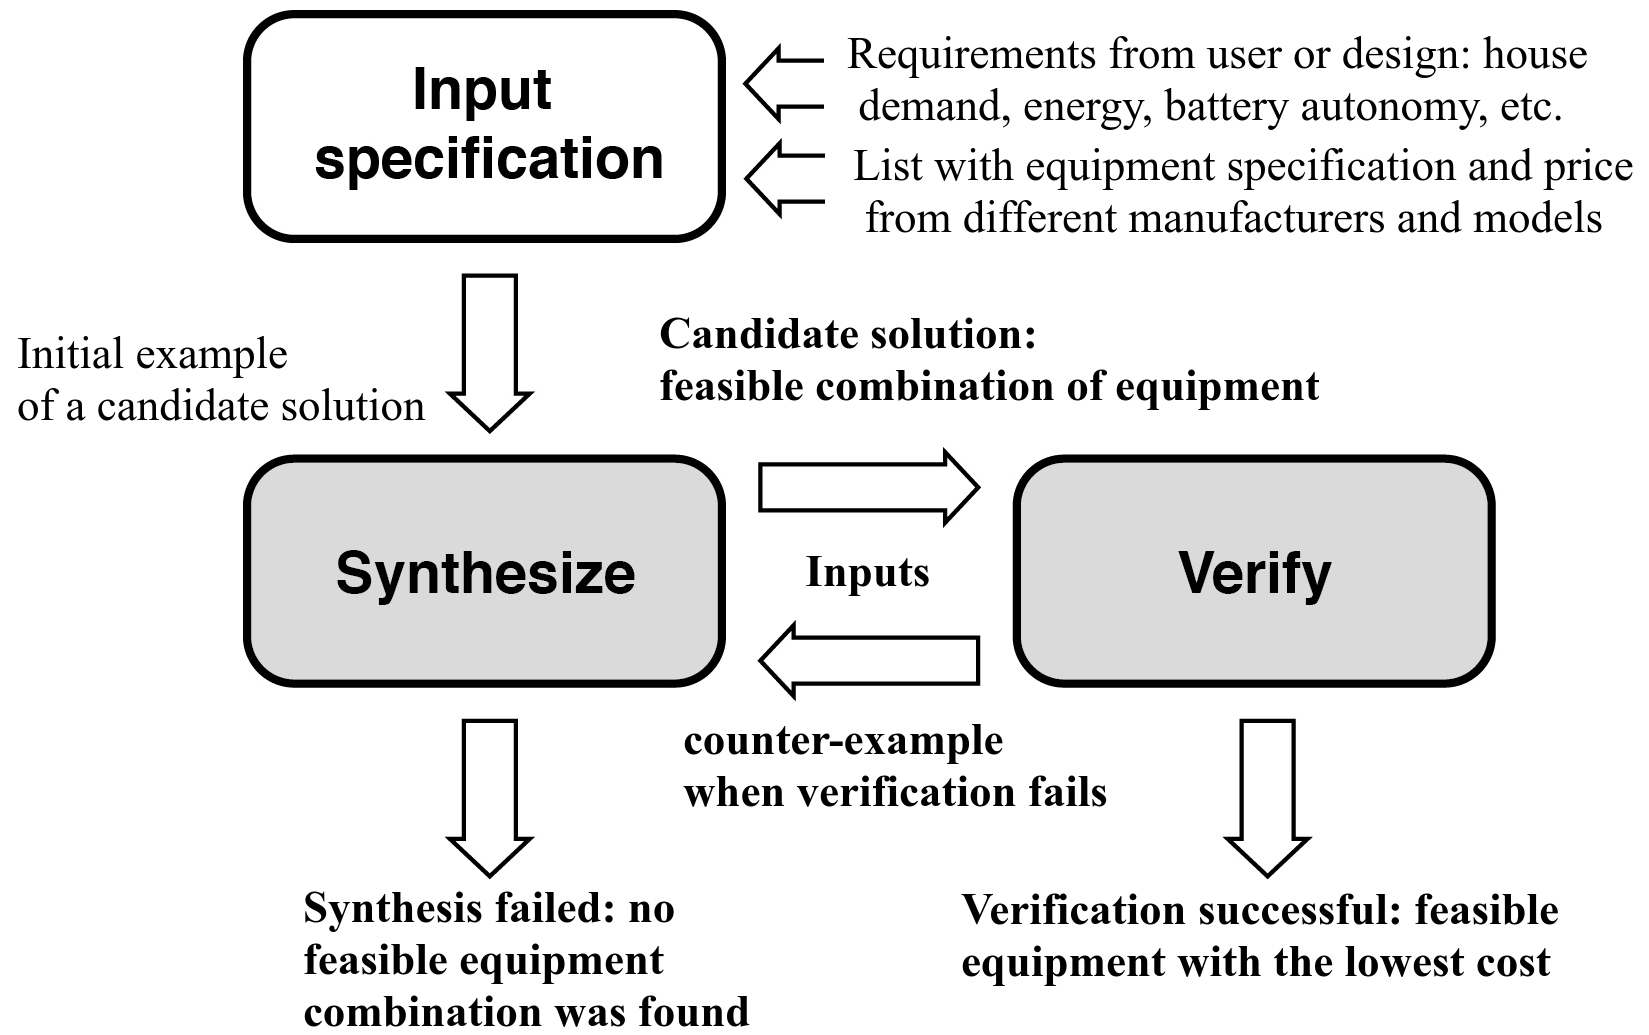
\includegraphics[width=0.75\columnwidth]{fig2_rev.jpg}
	\caption{CEGIS applied to PV system sizing.}
	\label{Counter-Example-Guided-Inductive-Synthesis}
\end{figure}

The correctness specification $\sigma$ provided to our program synthesizer is of the form $\exists \vec{F} .  \forall \vec{x}.  \sigma(\vec{x}, \vec{F})$, where $\vec{F}$ ranges over functions, $\vec{x}$ ranges over ground terms, and $\sigma$ is a quantifier-free (QF) formula typically supported by SMT solvers. The ground terms are interpreted over some finite domain $\mathcal{D}$, where $\mathcal{D}$ can be encoded using the SMT's bit-vectors part. Examples of specification used by our method include house demand, energy, and battery autonomy; we also provide a list of equipment specification and price from different manufacturers and models.

In Figure~\ref{Counter-Example-Guided-Inductive-Synthesis}, regarding traditional CEGIS method, the phases {\sc Synthesize} and {\sc Verify} interact via a finite set of test vectors {\sc inputs}, which is incrementally updated. Given the correctness specification $\sigma$, the {\sc Synthesize} procedure tries to find an existential witness $\vec{F}$ satisfying the specification $\sigma(\vec{x}, \vec{F})$, for all $\vec{x}$ in {\sc inputs} (as opposed to all $\vec{x} \in \mathcal{D}$). If {\sc Synthesize} succeeds in finding a witness~$\vec{F}$, the latter is a candidate solution (i.e., feasible combination of equipment) to the full synthesis formula, which is passed to {\sc Verify} in order to check whether it is a proper solution ({\it i.e.}, $\vec{F}$ satisfies the specification $\sigma(\vec{x}, \vec{F})$ for all $\vec{x}\in\mathcal{D}$). If this is the case, then the algorithm terminates, i.e., we have found a feasible equipment with the lowest cost; otherwise, in the CEGIS traditional method, additional information is provided to the phase {\sc Synthesize}, in the form of a new counterexample that is added to the {\sc inputs} set and the loop iterates again.

One may notice that each iteration of the traditional CEGIS loop adds a new input to the finite set $\text{\sc inputs}$, which is then used for synthesis.  Given that the full set of inputs $\mathcal{D}$ is finite because we use bit-vector expressions, this means that the refinement loop can only iterate over a finite number of times; however, {\sc Synthesize} may conclude that no candidate solution obeying $\sigma$ for the finite set $\text{\sc inputs}$ exists and our synthesis engine can then conclude that no feasible equipment combination was found.

However, in our variant CEGIS method proposed here, there are four particular differences related to the traditional CEGIS: 
(1) there exists no test vector and every candidate is generated during the run-time in the {\sc Synthesize} phase and sent to the {\sc Verify} phase; 
(2) if the {\sc Verify} phase is unsuccessful, then a new candidate is generated by {\sc Synthesize} and 
(3) the lower bound of the {\sc Verify} phase is incremented to search for the lowest cost; 
(4) as a result, there exists no refinement from the {\sc Verify} phase back to the {\sc Synthesize} phase, i.e., 
a new counterexample is not added to the {\sc input} set since a failure during the {\sc Verify} phase will only discard 
a given candidate that could be feasible in the next iteration with a new lower bound.

Program synthesis engines that implement the CEGIS approach~\cite{sketch} can automatically produce solutions for a large variety of specifications; here we have used symbolic software verifiers based on SMT solvers.

%%%%%%%%%%%%%%%%%%%%%%%%%%%%%%%%%%%%%%%%%%%%%%%%%%%%%%%%
\subsection{Sizing Stand-alone Solar PV Systems}
\label{sec:sizing}
%%%%%%%%%%%%%%%%%%%%%%%%%%%%%%%%%%%%%%%%%%%%%%%%%%%%%%%%

A PV system is illustrated in Fig.\ref{fig:blockdiagram}. It identifies the PV generator, batteries, charge controller, inverter, and AC load. 
The PV generator, which can be a panel or an array, is a semiconductor device that can convert solar energy into DC electricity.  
For night hours or rainy days, we hold batteries where power can be stored and used. The use of batteries as a storage 
form implies the presence of a charge controller~\cite{Hansen}. The PV arrays produce DC and therefore when the PV system 
contains an AC load, a DC/AC conversion is required. That converter is called inverter; and the AC load dictates the behavior 
of AC electrical load from the house that will be fed by the system.
%
\begin{figure}[h]
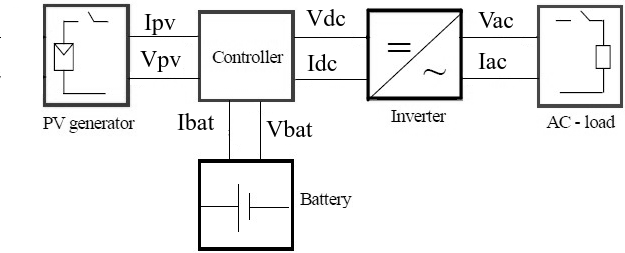
\includegraphics[width=0.7\textwidth]{blockdiagramPVS2_rev}
\centering
\caption{Block diagram for a typical stand-alone PV system~\cite{Hansen}.}
\label{fig:blockdiagram} 
\end{figure}

The sizing check stage will ensure that the system meets the standard project steps related 
to critical period solar energy method~\cite{Pinho} and adopting MPPT (Maximum Power Point Tracking) charge controller,
which is the most common one in practice. Firstly, we need to correct the energy consumption estimated to the load 
($E_{consumption}$), which is carried out by Eq.~\eqref{eq:Ecorrected}, where the efficiency of batteries ($\eta_{b}$), 
controller ($\eta_{c}$), and inverter ($\eta_{i}$) are considered~\cite{Pinho} as follows
%
\begin{equation}
\label{eq:Ecorrected}
E_{corrected} = \dfrac{E_{consumption}}{\eta_{b} \eta_{c} \eta_{i} }.
\end{equation}

We also need to estimate the energy that can be produced for each panel, called $E_{p}$, in Wh, defined as
%
\begin{equation}
\label{eq:Ep}
E_{p} = Solar\_Irradiance \times Panel\_Area \times \eta_{p} \times 1000,
\end{equation}

\noindent where the solar irradiance is expressed in terms of $kWh/m^{2}$ and depends on the site where the PV system will be deployed; 
the PV panel area is given in $m^{2}$ and corresponds to the size of one PV panel, and $\eta_{p}$ represents the PV panel efficiency.
The total minimum number of needed solar panels ($N_{TPmin}$) is computed as
%
\begin{equation}
\label{eq:NTPmin}
N_{TPmin} = \dfrac{E_{corrected}}{E_{p}}.
\end{equation}

Particularly, the total number of panels in series ($N_{PSmin}$) and parallel ($N_{PPmin}$) are respectively given by
%
\begin{equation}
\label{eq:NPSmin}
\dfrac{V_{mppt,min}}{V_{maxPower,TempMax}} \leq N_{PSmin} \leq \dfrac{V_{mppt,max}}{V_{maxPower,TempMin}},
\end{equation}
%
\begin{equation}
\label{eq:NPPmin}
N_{PPmin} = \dfrac{P_{total}}{Number\,Panels\,Series \times P_{max,ref}},
\end{equation}
%
\noindent where $V_{mppt,max}$ is the maximum operation voltage and $V_{mppt,min}$ 
is the minimum operation voltage of the charge controller; $V_{maxPower,TempMax}$ and 
$V_{maxPower,TempMin}$ are the maximum power voltage from the PV module considering 
the maximum and minimum operational temperature, respectively; 
$P_{total}$ is the total power demanded from the PV system and 
$P_{max,ref}$ is the power supplied from one PV panel in $Watts$.
Regarding batteries, we must first define the total capacity of the battery bank, which can be described as
%
\begin{equation}
\label{eq:Cbank}
C_{bank} = \dfrac{E_{corrected} \times autonomy}{V_{system} \times DOD},
\end{equation}

\noindent where the variable $autonomy$ is a design definition and normally has a value ranging from $6$ to $48$h; 
$ V_{system} $ is the DC voltage of the bus, and $ DOD $ is the battery deep of discharge (considered of maximum of 25\% here).
%
Secondly, the total (minimum) number of batteries is computed as 

\begin{equation}
\label{eq:Nbtotal}
N_{B}total = N_{BS}min \times N_{BP}min = \dfrac{V_{system}}{V_{bat}} \times \dfrac{C_{bank}}{1 \,Battery \, Capacity}.
\end{equation}

Regarding the charge controller, it must initially meet the voltage requirement of the PV system, as described by Eq.~\eqref{eq:vcvsystem} to the charge controller voltage: 
\begin{equation}
\label{eq:vcvsystem}
V_{c} = V_{system}.
\end{equation}

The short circuit reference information from the manufacturer's solar panel must be corrected 
to the cell temperature because the field temperature is higher than the nominal or laboratory temperature, 
and PV system is temperature dependent, as 
%
\begin{equation}
\label{eq:iscamb}
I_{sc,amb} = \dfrac{G}{G_{ref}} \left[ I_{sc,ref} + \mu_{I} \times (T-25) \right]. 
\end{equation}

The controller must meet the maximum current from the PV array given by Eqs.~\eqref{eq:icmin} and~\eqref{eq:icicmin} as
%
\begin{equation}
\label{eq:icmin}
I_{c,min} = I_{sc,amb} \times N_{PP},
\end{equation}
%
\begin{equation}
\label{eq:icicmin}
I_{c} \geq I_{c,min}.
\end{equation}

The inverter sizing check is performed by means of three equations. Eq.~\eqref{eq:vindc} ensures that 
the input voltage of the controller meets the system voltage. Eq.~\eqref{eq:voutac} ensures that the 
output voltage of the controller meets the AC voltage of the load. Finally, Eq.~\eqref{eq:invcheck} ensures that 
the controller can support the total demand of the load ($Demand$) and the surge power ($P_{surge}$), 
where $V_{in}DC$ is the nominal input voltage and $V_{out}AC$ is the nominal output voltage of the inverter; 
$MAX_{AC,ref}$ is the peak power that the inverter can support.
%
\begin{equation}
\label{eq:vindc} 
V_{in}DC = V_{system}.
\end{equation}
%
\begin{equation}
\label{eq:voutac} 
V_{out}AC = V_{AC}.
\end{equation}
%
\begin{equation}
\label{eq:invcheck} 
\left[ (Demand \leq P_{AC,ref}) \, and \, (P_{surge} \leq MAX_{AC,ref}) \right].
\end{equation}

%%%%%%%%%%%%%%%%%%%%%%%%%%%%%%%%%
\subsection{PV systems Optimization Criteria}
%%%%%%%%%%%%%%%%%%%%%%%%%%%%%%%%%

In order to select an optimal combination to meet sizing constraints, 
it is necessary to evaluate power reliability and system cost analysis for the underlying system. An ideal combination of any PV system is made by the best compromise between these two objectives.

During the PV system design, one of the most important aspects to ensure power system reliability is to analyze power supply availability~\cite{Alsadi2018}. The reason is because solar energy production is intermittent and, therefore, the energy generated usually will not match with the load demand. A reliable power is a generation system that has sufficient power to feed load demand in a period. 

There exist different methods to express system reliability, where the most popular ones 
are the loss of load probability (LOLP) and the loss of power supply probability (LPSP)~\cite{Alsadi2018}. In both methods, if the probability is zero, then the load will always be fulfilled; otherwise (i.e., probability of one) the load will never be fulfilled.

LOLP is the probability for the case when a load demand exceeds the generation power by the PV system. On one hand, we claim that we have a reliable PV system when it is able to generate sufficient power to fulfill the demanded load within a time span. On the other hand, LPSP is defined as the probability of the case when system generates insufficient power to satisfy the load demand. The main approaches to LPSP demand simulation or probabilistic treatment of time series data to predict dynamic changing on system performance. However, data is not always available and dynamic analysis is complex; and this is a drawback of LOLP and LPSP~\cite{Alsadi2018}.

Related to economic analysis, there exist various methods available. The main objective is to determine whether the project has an acceptable investment; the usual way is to perform economic analysis after reliability analysis with the goal of proposing a system with high reliability and lowest cost~\cite{Alsadi2018}. The common methods include: Net Present Cost (NPC)~\cite{Park2004}, the Levelized Cost of Energy (LCOE)~\cite{Zhou2010}, or the Life Cycle Cost (LCC)~\cite{Applasamy2011}.

The NPC is the present value of all the costs over the project lifetime, minus the present value of all the revenues that it earns over the project lifetime. The net present worth is found by discounting all cash inflows and outflows, including cost of installation, replacement and maintenance of the PV system, at an internal rate of return (IRR)~\cite{Park2004}. IRR is used to evaluate the attractiveness of a project or investment.

LCOE is defined as the average cost per kWh of useful electrical energy produced by the PV system when a lifetime, investment cost, replacement, operation and maintenance, and capital cost are considered~\cite{Kamel2005}. LCOE method is useful in comparing different generation technologies with different operating characteristics~\cite{Zhou2010}.

LCC is the estimation of sum of installation cost, operating and maintenance of a PV system for a period of time, and expressed in today's value~\cite{Applasamy2011}. Eq.~\eqref{eq:LCC} is used to calculate LCC of a PV system,
%
\begin{equation}
\label{eq:LCC}
LCC = C_{PV} + C_{bat} + C_{charger} + C_{inv} + C_{installation} + C_{batrep} + C_{PWO\&M},
\end{equation}
\noindent where $C_{PV}$ is PV array cost, $C_{bat}$ is initial cost of batteries, $C_{charger}$ is cost of charger, $C_{inv}$ is inverter cost, $C_{installation}$ is installation cost, $C_{batrep}$ is battery replacement cost in present value, and $C_{PWO\&M}$ is operation and maintenance costs 
in present worth.

%----------------------------------------------------------------------------------------------
\subsection{Stand-alone PV System Optimization Technique}
%----------------------------------------------------------------------------------------------

In order to recommend an optimal configuration for PV systems, 
the designer has to evaluate the design based on optimization variables. 
As the number of optimization variables increases, the computational effort 
will increase as well. Hence, to obtain the best PV system design as well as 
simplified sizing process, prior work introduced three main techniques 
for system sizing calculation, namely intuitive, numerical, and analytical methods~\cite{Zhou2010}.

Intuitive method is simple, easy to be implemented, and can be used to give 
rough suggestion for preliminary design. The sizing rules are based on designer's experience, 
using lowest performance either in a time period data or by directly using average value 
(daily, monthly, or annual) of solar irradiance. This method does not consider the battery's 
state of charge, or even the random nature of solar irradiation and meteorological conditions~\cite{Alsadi2018}.

For numerical method, the design is simulated for each time step within a period. 
State of charge of batteries is calculated and investigated. It is very accurate, 
however is complex, demanding more time for calculation~\cite{Park2004}.

Analytical methods is used to obtain a close relation or correlation in a form 
of equation between capacities and reliabilities. The sizing task becomes much simpler 
than numerical technique; however, the relation cannot be applied to different sites
since it is specific to one place of deployment of the PV system, 
thereby demanding adaptation if another site is analyzed.

%------------------------------------------------------
\section{SYNTHESIZING OPTIMAL SIZING OF STAND-ALONE SOLAR PHOTOVOLTAIC SYSTEMS}
\label{sec:Method}
%------------------------------------------------------

Algorithm~\ref{alg:verification-algorithm} describes our pseudo-code to synthesize stand-alone PV systems using symbolic model checking. It was adopted the analytical method of optimization, with LCC economical analysis and power reliability based on the critical period criteria.
%
 \begin{algorithm}
 \caption{Synthesis algorithm}
 \begin{algorithmic}[1]
 \renewcommand{\algorithmicrequire}{\textbf{Input:}}
 \renewcommand{\algorithmicensure}{\textbf{Output:}}
  \STATE Initialize variables \\
  \STATE Declare list of PV panels, controllers, batteries, and inverters data and cost \\
%  \STATE Declare list of controllers data and cost \\
%  \STATE Declare list of batteries data and cost \\
%  \STATE Declare list of inverters data and cost \\
  \STATE Declare the maximum possible cost $MaxCost$  \\
  \STATE Declare power demand, power peak, energy consumption \\
  \STATE Declare battery autonomy, deep of discharge, AC voltage \\
  \FOR {$HintCost=0$ to $MaxCost$}
 	\STATE Declare non-deterministic variable to select PV Panel from list \\
 	\STATE Declare non-deterministic variable to select Controller from list \\
 	\STATE Declare non-deterministic variable to select Battery from list \\
 	\STATE Declare non-deterministic variable to select Inverter from list \\ 	
 	\STATE Calculate $E_{corrected}, \, E_{p} $ \\
	\STATE Calculate $N_{TPmin}, \, N_{PSmin}, N_{PPmin} $ \\
 	\STATE Calculate $C_{bank}$ \\
	\STATE Calculate $N_{BS}min, \, N_{BP}min, \, N_{B}total$ \\
	\STATE Requirement enforced by \textbf{assume}$(V_{c})$ \\
 	\STATE Calculate $I_{sc,amb}$ \\
 	\STATE Calculate $I_{c,min}$ \\
 	\STATE Requirement enforced by \textbf{assume}$(I_{c} \wedge V_{in}DC \wedge V_{out}AC)$ \\
%	\STATE Requirement enforced by \textbf{assume}$(V_{in}DC \wedge V_{out}AC )$ \\
%	\STATE Requirement enforced by \textbf{assume}$(V_{out}AC)$ \\
	\STATE Requirement enforced by \textbf{assume}$(Demand \wedge P_{surge})$ \\
%	\STATE Requirement enforced by \textbf{assume}$(P_{surge})$ \\
	\STATE non-deterministic variables hold feasible equipment and cost  \\
	\STATE $F_{obj} \leftarrow  N_{TP}*Panel_{Cost} \, + \, N_{TB}*Battery_{Cost} \, + Controller_{Cost} \, + \, Inverter_{Cost} \, + \, Installation_{Cost} \, + \, batrep_{Cost} \, + \, PWO\&M_{Cost}$ \\
	\STATE Violation check with \textbf{assert}$(F_{obj} > HintCost)$ \\
  \ENDFOR
 \RETURN $(\,)$ 
 \end{algorithmic} 
 \label{alg:verification-algorithm}
 \end{algorithm}
%

Our synthesis algorithm will synthesize constant values; 
it starts with the input of manufacturers data and prices of PV panels, batteries, 
charge controllers and inverters (line $2$). After that, we define user requirements, i.e., 
house requirements and design definitions, from lines $4$ and $5$. 

The \textit{for}-loop started at line $6$ controls the lowest cost to the PV solution. 
In particular, it starts with cost $0$ and stops only when the algorithm finds a 
feasible solution in which the cost breaks the $assertion$ stated in line $22$; 
if that happens, then our algorithm has found an optimal solution, thereby stating 
that the {\sc Verify} phase reached a satisfiable condition (\textit{SAT}). 
The $MaxCost$ value at line $6$ is just a very high value put as a limit 
to the \textit{for}-loop, that never will be reached because the optimal solution will be found first.

Our synthesis algorithm uses non-deterministic variables to choose one specific constant 
from a given list of PV panels, controllers, batteries and inverters (lines $7$ to $10$). 
That procedure ensures that our synthesis engine checks all combinations of items 
from each equipment, and combine them to assemble a feasible (candidate) PV solution, 
which meets the user requirements.

Next, we use Eq.~\eqref{eq:Ecorrected}, Eq.~\eqref{eq:Ep}, Eq.~\eqref{eq:NTPmin}, 
Eq.~\eqref{eq:NPSmin}, Eq.~\eqref{eq:NPPmin}, Eq.~\eqref{eq:Cbank}, 
Eq.~\eqref{eq:Nbtotal}, Eq.~\eqref{eq:iscamb}, and Eq.~\eqref{eq:icmin} t
o calculate the sizing variables (lines $11$ to $17$). The directive \textit{assume} (lines $15$, $18$ and $19$) 
ensures the compatibility of the chosen items from the list of equipment: the {\sc Verify} phase 
uses only the item (among all the possible ones) that satisfies the statements of Lines $15$, $18$ and $19$. 
Therefore, our synthesis algorithm reaches line $20$ with one feasible solution, 
and the cost of that solution is calculated in $F_{obj}$ (line $21$). 

If our algorithm does not find a feasible solution among the item of equipment that 
were provided to our {\sc Synthesize} phase,  then the result is an unsatisfiable (\textit{UNSAT}), i.e., 
the program finishes and does not find a solution, which indicates that it 
was not possible to combine the items of each equipment in order to create a feasible solution. 

The main challenge for the {\sc Synthesize} phase is to find a feasible candidate 
solution regarding the constraints and user requirements. Related to our {\sc Verify} 
phase the challenge is to find the lowest acquisition cost from a list of equipment and 
components that is provided from the {\sc Synthesize} phase. 

Note that the process described here in completely automated and that a validation is performed 
by our {\sc Verify} phase to ensure that the approach is sound.

%%%%%%%%%%%%%%%%%%%%%%%%%%%%%%%
\subsection{Assumptions and Premises}
%%%%%%%%%%%%%%%%%%%%%%%%%%%%%%%

Regarding the line $2$ of Algorithm~\ref{alg:verification-algorithm}, 
a list of forty equipment from ten different manufacturers was provided 
to the synthesis engine in order to allow the choice of every item 
of PV sizing. Data sheet from each item was necessary to collect 
technical information. Moreover, the price of each item was obtained 
from available quotations in the market, and if the currency was not in US dollars, 
then it was used the exchange rate of the day to convert it to US dollars.

With respect to power reliability, this work will rely on the critical period solar 
energy method~\cite{Pinho} as described in Section~\ref{sec:sizing}. 
The usual way is to use loss of load probability (LOLP) or loss of power 
supply probability (LPSP). However, based on the fact that here we 
are neither considering site characteristics nor the load changes over time, 
which demands historical data, the reliability analysis will be developed only 
by the critical period method of PV sizing.

Regarding financial analysis:
\begin{itemize}
	\item LCC lifetime considered: $20$ years;
	\item Installation costs: includes delivery in the isolated community and installation costs itself, $5$\% of total cost~\cite{Agrener2013};
	\item Value of the discount rate or interest rate: $10$\%, which is a good rate considering financial investments in developing countries;
	\item Operation and maintenance annual costs: based on past PV projects of similar size in the Amazon region of Brazil, will be adopted the value of US\$ 289.64~\citep{Agrener2013}. This cost includes the battery replacement based on its lifetime ($4$ years for lead-acid batteries), plus inverters and controller replacement (every $10$ years). Therefore, it will be performed three battery bank and one inverter-controller replacements during the LCC analysis.
\end{itemize}

On the subject of PV system optimization technique, we will adopt here the intuitive method 
since the average value daily of solar irradiance is used in the mathematical model, 
without considering the battery's state of charge, or even the random nature 
of solar irradiation and meteorological conditions. Therefore, all the computational 
effort will be concentrated in our automated synthesis algorithm.

Regarding all case studies, it was defined that the minimum state of charge of batteries is $75$\% (with DOD maximum of $25$\%, which is common to lead-acid batteries), the voltage of the system is set in $24$ V DC (the most common as well, but the value can be adjusted to $12$ or $48$ V at the code), and the AC voltage from the inverter is $127$ V (Brazilian standard).

Related to off-the-shelf simulation tools only HOMER Pro and Hybrid2 perform off-grid system with battery backup analysis. Additionally, HOMER and RETScreen include economical analysis or even optimization-sensitive analysis. Therefore, in this study, HOMER Pro will be the simulation tool used to compare with our automated synthesis method.  Related to HOMER Pro:

\begin{itemize}
	\item HOMER Pro is available only for Microsoft Windows and its annual standard subscription costs US\$ $504.00$~\cite{HOMER};
	\item HOMER Pro do not have the LCC cost in its reports. However, it has NPC and LCOE. Therefore NPC was used to obtain LCC in order to allow the comparative among tools;
	\item The optimization analysis of HOMER Pro allows to define a load curve and temperature according of data collected automatically from online databases. However, in order to allow a correct comparative, the curve load and the temperature were defined exactly the same as automated synthesis tools;
	\item Battery autonomy is not an parameter that the user can set when using HOMER Pro. The tool will always to meet the user requirement, i.e., the load curve during the $365$ days of the year;
	\item HOMER Pro do not have a explicit equipment called charge controller. It uses a controller resource that can perform in two different ways, according of the optimization choice or the user choice: load following or cycle charging~\cite{HOMER}. During the tests it was chosen the load following controller: it produces only enough power to meet the demand~\cite{HOMER};
	\item It was assumed the value of 5\% of capacity shortage that is equivalent to 95\% of availability of the PV system. By definition, availability is the percentage of time at which a power system is capable of meeting the load requirements~\citep{Khatib2014}. For critical loads, 99\% is considered acceptable. While in a ordinary house electrical load, 95\% is considered acceptable;
	\item It was assumed a string of two batteries in order to match the voltage of the system of $24$ V DC that was used for the automated synthesis tool;
	\item The premise adopted when using HOMER Pro it was that the user does not know the optimal solution, and that in order to obtain this solution is necessary to include (at the design phase of the tool) generic PV and batteries modules that HOMER Pro will search for the optimized power of each component. With that in mind, it was included a generic flat plate PV of $1$ kW and generic lead-acid batteries of $1$ kW as well (and with capacity of $83.4$ Ah according with HOMER Pro modeling). HOMER, during run-time, decides the size in kW of each module, based on feasibility and lower cost.
\end{itemize}

%---------------------------------------------------------------------------
\section{EXPERIMENTAL EVALUATION}
\label{sec:Results}
%---------------------------------------------------------------------------

This section presents the case studies used to evaluate our proposed approach. 
We also compare our approach with a simulation tool, named HOME Pro. 
The version and command-line of each verifier adopted, 
the computing setup, the objectives of the experimental phase, 
and the results itself are also described.

%---------------------------------------------------------------------------
\subsection{Case studies} 
%---------------------------------------------------------------------------

We have performed seven stand-alone PV system case studies to evaluate 
our proposed synthesis approach, as described in the first column of 
Table~\ref{tab1} (named Specification). These case studies were defined 
based on usual electrical load found in riverside communities of the 
Amazon State in Brazil~\cite{abs-1811-09438, Agrener2013}. 
%
\begin{table}
\caption{Case studies and results: optimization of stand-alone PV systems.}\label{tab1}
\begin{scriptsize}
\begin{tabular}{|c|c|c|c|c|}
\hline
\hline
Tools & \makecell{CBMC 5.11 \\(MiniSat 2.2.1)}& \makecell{ESBMC 6.0.0 \\(Boolector 3.0.1 /\\Z3 4.7.1)}& \makecell{CPAchecker 1.8\\(MathSAT 5.5.3)}& HOMER Pro 3.13.1\\
\hline
\hline
Specification & Result & Result & Result & Result \\
\hline
\makecell{\textbf{Case Study 1}\\Peak:342W\\Surge:342W \\E:3,900Wh/day\\Autonomy:48h} & OM & TO / IF & \makecell{SAT (172.03 min) \\NTP:1$\times$340W (1S)\\NBT:8$\times$105Ah (2S-4P)\\Controller 15A/75V\\Inverter 700W/48V\\LCC: US\$ 7,790.53} & \makecell{(Time: 0.33 min)\\2.53 kW of PV\\NBT:12$\times$83.4Ah (2S-6P)\\0.351kW inverter\\LCC: US\$ 7,808.04}\\
\hline
\makecell{\textbf{Case Study 2}\\Peak:814W\\Surge:980W\\E:4,880Wh/day\\Autonomy:48h} & OM & TO / IF & \makecell {SAT (228.7 min) \\NTP:2$\times$330W (2S)\\NBT:10$\times$105Ah (2S-5P)\\Controller 20A/100V DC\\Inverter 1,200W/24V \\LCC: US\$ 8,335.90} & \makecell{(Time: 0.18 min)\\3.71 kW of PV\\NBT:20$\times$83.4Ah (2S-10P)\\0.817kW inverter\\LCC: US\$ 12,861.75} \\
\hline
\makecell{\textbf{Case Study 3}\\Peak:815W\\Surge:980W\\E:4,880Wh/day\\Autonomy:12h} & OM & TO / IF & \makecell {SAT (166.13 min) \\NTP:4$\times$150W (4S)\\NBT:4$\times$80Ah (2S-2P)\\Controller 15A/100V DC\\Inverter 1,200W/24V \\LCC: US\$ 7,306.27} & Not possible \\
\hline
\makecell{\textbf{Case Study 4}\\Peak:253W\\Surge:722W\\E:3,600Wh/day\\Autonomy:48h} & OM & TO / IF & \makecell {SAT (143.71 min) \\NTP:4$\times$150W (4S)\\NBT:10$\times$80Ah (2S-5P)\\Controller 15A/75V\\Inverter 750W/24V \\LCC: US\$ 7,816.31} & \makecell{(Time: 0.23 min)\\2.42 kW of PV\\NBT:12$\times$83.4Ah (2S-6P)\\0.254kW inverter\\LCC: US\$ 7,677.95}\\
\hline
\makecell{\textbf{Case Study 5}\\Peak:263W\\Surge:732W\\E:2,500Wh/day\\Autonomy:48h} & OM & TO / IF & \makecell {SAT (134.93 min) \\NTP:1$\times$340W (1S)\\NBT:6$\times$105Ah (2S-3P)\\Controller 15A/75V\\Inverter 400W/24V \\LCC: US\$ 7,252.14} & \makecell{(Time: 0.18 min)\\1.59 kW of PV\\NBT:10$\times$83.4Ah (2S-5P)\\0.268kW inverter\\LCC: US\$ 6,175.57} \\
\hline
\makecell{\textbf{Case Study 6}\\Peak:322W\\Surge:896W\\E:4,300Wh/day\\Autonomy:48h} & OM & TO / IF & \makecell {SAT (235.75 min) \\NTP:2$\times$200W (2S)\\NBT:10$\times$105Ah (2S-5P)\\Controller 15A/75V\\Inverter 400W/24V \\LCC: US\$ 8,287.23} & \makecell{(Time: 0.22 min)\\3.15 kW of PV\\NBT:14$\times$83.4Ah (2S-7P)\\0.328kW inverter\\LCC: US\$ 9,112.45} \\
\hline
\makecell{\textbf{Case Study 7}\\Peak:1,586W\\Surge:2,900W\\E:14,000Wh/day\\Autonomy:48h} & OM & TO / IF & TO & \makecell{(Time: 0.20 min)\\12.5 kW of PV\\NBT:66$\times$83.4Ah (2S-33P)\\1.60kW inverter\\LCC: US\$ 41,878.11} \\
\hline
\hline
\end{tabular}
\\Legend: OM = out of memory; TO = timeout; IF = internal failure, E = energy.
\end{scriptsize}
\end{table}


%---------------------------------------------------------------------------
\subsection{Tools} 
%---------------------------------------------------------------------------

Three start-of-art verification tools, CBMC\footnote{Command-line: \$ cbmc -\phantom{}-unwind 100 filename.c -\phantom{}-trace}, ESBMC\footnote{Command-line: \$ esbmc filename.c -\phantom{}-no-bounds-check -\phantom{}-no-pointer-check -\phantom{}-unwind 100 -\phantom{}-boolector}, %UAutomizer\footnote{Command-line: \$ ./Ultimate -tc config/AutomizerReach.xml -s config/svcomp-Reach-32bit-Automizer\_Default.epf -i filename.c -\phantom{}-traceabstraction.limit.analysis.time 900 -\phantom{}-traceabstraction.stop.after.first.violation.was.found false -\phantom{}-cacsl2boogietranslator.overapproximate.operations.on.floating.types false -\phantom{}- cacsl2boogietranslator.assume.nondeterminstic.values.are.in.range false -\phantom{}-rcfgbuilder.add.additional.assume.for.each.assert true -\phantom{}-rcfgbuilder.simplify.code.blocks true -\phantom{}-rcfgbuilder.size.of.a.code.block LoopFreeBlock}, 
and CPAchecker\footnote{Command-line: \$ scripts/cpa.sh -heap 64000m -config config/bmc-incremental.properties -spec config/specification/sv-comp-reachability.spc filename.c} were used as our verification engine to compare our approach effectiveness and efficiency. Note that ``incremental'' ESBMC with the SMT solver Z3 was tried\footnote{Command-line: \$ esbmc filename.c -\phantom{}-no-bounds-check -\phantom{}-no-pointer-check -\phantom{}-unwind 100 -\phantom{}-smt-during-symex -\phantom{}-smt-symex-guard -\phantom{}-z3} as an alternative to use less computing memory. The Simulation tool HOMER Pro version $3.13.1$ was used for comparative purpose.

%---------------------------------------------------------------------------
\subsection{Setup} 
%---------------------------------------------------------------------------

All experiments regarding the verification tools were conducted 
on an otherwise idle Intel Xeon CPU E5-4617 ($8$-cores) with 
$2.90$ GHz and $64$ GB of RAM, running Ubuntu $16.04$ LTS $64$-bits. 
Related to HOMER Pro, we have used an Intel Core i5-$4210$ ($4$-cores), 
with $1.7$ GHz and $4$ GB of RAM, running Windows 10. 
Our experiments were performed with a predefined timeout of $240$ minutes.

%---------------------------------------------------------------------------
\subsection{Objectives} 
%---------------------------------------------------------------------------

Our evaluation aims to answer two experimental questions: 

\begin{enumerate}

\item[EQ1] \textbf{(soundness)} does our automated synthesis approach provide correct results?

\item[EQ2] \textbf{(performance)} how do the software verifiers compare to each other?

\end{enumerate}

%---------------------------------------------------------------------------
\subsection{Results}  
%---------------------------------------------------------------------------

CPAchecker was able to synthesize the optimal sizing in six 
out of seven case studies: the result was produced within 
the time limit, which varied from $134.71$ to $235.75$ minutes. 
Only case study $7$ led to a \textit{timeout} result, i.e., 
it was not solved within $240$ minutes. However, if we remove 
this timeout limitation from CPAchecker, the verifier is 
able to solve the optimization in $44.97$ hours. 
The violation (SAT result) indicated in Table~\ref{tab1} 
is the $assert$ of line $22$ from Algorithm~\ref{alg:verification-algorithm}. %The results were tested by manual PV sizing and were sound (\textit{RQ1}). %, linking a feasible technical solution with the lowest cost possible, considering the equipment that were inputted to the code. 

CBMC and ESBMC are unable to produce any conclusive result. 
Situations of \textit{internal failure}, \textit{timeout}, 
or \textit{out of memory} occurred; this partially answers 
the \textit{EQ2}. Note that the internal failure presented 
by ESBMC was a Z3 solver issue (a bug); this will demand 
an updated version of ESBMC to fix this issue. Similarly to CPAchecker, 
if we remove the timeout from ESBMC with the SMT solver Boolector, 
then the verifier is able to obtain the automated synthesis 
in $73.18$ hours for the case study $2$. CBMC, in the other hand, only could present some result if the RAM memory of the system was bigger to avoid the memory out issue.

Related to HOMER Pro, it was able to evaluate six case studies, 
and within a time shorter than $30$ seconds, which was much 
faster than our automated synthesis tool (cf.~\textit{EQ2}). 
Case study $3$ was not possible to be simulated since HOMER Pro 
does not have the feature of adjusting the battery autonomy, i.e., 
the tool always tries to feed with electricity the given load 
during $365$ days/year. We have also noted other HOMER Pro drawbacks:

\begin{itemize}
\item There exists no explicit charge controller 
as a system equipment. HOMER Pro includes automatically 
a controller just to simulate the charge/discharge 
of batteries and to meet the load requirement; however, 
without costs or even with electrical characteristics 
as maximum current and voltage, which are common during PV sizing;
\item HOME Pro demands to include some battery specification 
to initiate the optimization; however, it does not change 
the electrical specifications during the simulation; 
the presented results are multiples of the original 
battery type suggested by the user. As example, it was 
started with a $83.4$ Ah lead-acid battery and during 
the simulation, HOMER Pro did not try to use other capacities or types;
\item HOMER Pro does not present the optimal solution 
in terms of connections of arrays of PV panels, just the 
total in terms of power, i.e., it does not present neither models 
and the power of each PV panel nor the total of panels in series or parallel. 
\end{itemize}

%%%%%%%%%%%%%%%%%%%%%%%%%%%%%%%%%%%%%%%%%%%%%%%%%%%%%%%%%%%%%%%%%%%%
\subsection{Comparison between Formal Synthesis and HOME Pro}
%%%%%%%%%%%%%%%%%%%%%%%%%%%%%%%%%%%%%%%%%%%%%%%%%%%%%%%%%%%%%%%%%%%%

Comparing the results between the formal synthesis with CPAchecker 
and HOMER Pro, we observed that most results are quite similar, 
in terms of technical solution and cost (cf. Table~\ref{tab1}). 

Particularly related to LCC, the cost was very close in cases 
$1$, $4$, $5$ and $6$, with difference varying from $0.23$\% to $17.4$\%. 
Even adopting the same price per kW to the PV panels, 
inverters, and batteries, HOMER Pro does not use costs 
related to charge controllers, which were introduced into the 
CPAchecker modeling. The premise used in CPAchecker to adopt 
a fixed annual cost for operation and maintenance can produce 
some impact as well at this discrepancy; however, it is not significant
since this annual cost is too small when compared to the resulting LCC value.

However, there exists a huge divergence in case study $2$, 
where the costs presented by HOMER Pro were $54$\% higher 
than our automated synthesis tool, probably because the 
operation and maintenance costs assumed by our automated 
synthesis tool were underestimated to that specific load. 

In general, the size of the PV panels and battery bank were 
bigger in HOMER Pro than with our formal synthesis approach, 
and that discrepancy is not easy to address without some real 
systems validation. The mathematical models are different and 
particular parameters can be tuned as well in each approach, 
and that can justify the difference, which was presented in all 
the case studies. As comparative, let's consider case study $1$: 
the optimal solution provided by HOMER Pro demands $7$ $\times$ 
more PV panels than the solution presented by our synthesis tool, 
and HOME Pro does not show the arrangement of arrays 
(i.e., the number of series and parallel PV panels); 
the battery bank presented by HOMER Pro provides $500.4$ Ah 
of capacity ($6 \times 83.4$), while our synthesis tool 
presented an optimal solution with $420$ Ah of total capacity 
($4 \times 105$). 

Just to compare the results obtained from the optimization 
with the real-world, the authors had four PV systems deployed 
and monitored since June $2018$ in a riverside community 
in the Amazonas State in Brazil, with similar demands 
presented by case studies $1$, $4$, $5$, and $6$, 
always with a $3$ $\times$ $325$ W ($3$S) panels and 
$4$ $\times$ $220$ Ah ($2$S-$2$P $= 440$ Ah) 
lead-acid batteries. These solutions are more close 
to the result presented by our formal synthesis 
approach than HOMER Pro, thereby showing that our 
solution is sound, which answers \textit{EQ1}.

Related to the inverters, HOMER Pro suggests a value in 
kW very close to the peak of every case study, and it 
is just a reference value and not a commercial value of 
the employed inverter. Our synthesis tool, however, 
presents inverters that are commercial and can be found 
off-the-shelf. Therefore is a PRO to the formal synthesis method.

Concerning to charge controllers, as we reported in 
the previous section, HOMER Pro does not include it 
as an explicit equipment in its mathematical model, 
only our synthesis tool presents a commercial controller 
and includes it during the cost analysis. Therefore, 
the formal synthesis method presents more reliable results than
HOME Pro.

Case study $7$ was not solved by our synthesis tool 
within the time limit established during the experimental 
phase. Case study $3$ was not possible to simulate in HOMER Pro, 
because its restriction does not allow one to set the battery autonomy, 
thus resting both without parameters to comparative.

Summarizing, our synthesis tool is capable to present a 
solution, which is far detailed and close to the commercial 
reality than the solution presented by HOMER Pro. 
In particular, our automated synthesis method 
can provide all the details of every component of 
a PV system solution, with complete electrical details 
from data sheet of manufacturers, including 
the model of the component, nominal current and voltage. 
In this respect, even the name of the manufacturer 
can be presented (in Table~\ref{tab1} it was removed 
to avoid some advertising).
%used with the SMT incremental mode\footnote{Command-line: \$ esbmc filename.c -\phantom{}-no-bounds-check -\phantom{}-no-pointer-check -\phantom{}-unwind 100 -\phantom{}-smt-during-symex -\phantom{}-smt-symex-guard -\phantom{}-z3} enabled with the goal of reducing memory usage; we have also used the SMT solver Z3 version 4.7.1~\cite{DeMoura}.

%%%%%%%%%%%%%%%%%%%%%%%%%%%%%%%%%%%%%%%%%%
\subsection{Threats to validity}
%%%%%%%%%%%%%%%%%%%%%%%%%%%%%%%%%%%%%%%%%%

We have reported a favorable assessment of our formal synthesis method. 
Nevertheless, we have also identified three threats to the validity 
of our experimental results, which can be further assessed and 
constitute future work: ($1$) improvement of the power reliability 
analysis: to include loss of load probability or loss of power 
supply probability, which can make the analysis more accurate; 
($2$) the cost analysis is well tailored to the Amazon region of Brazil; 
however, a broad analysis from other isolated areas must be 
performed in order to make the optimization general in terms 
of applicability; ($3$) to deploy at the field some PV systems 
sized using our synthesized results in order to validate it.

%%%%%%%%%%%%%%%%%%%%%%%%%%%%%%%%%%%%%
\section{CONCLUSIONS}
\label{sec:Conclusion}
%%%%%%%%%%%%%%%%%%%%%%%%%%%%%%%%%%%%%

We have described and evaluated an automated synthesis method 
to obtain the optimal size of PV system using software model 
checking techniques. \textcolor{red}{The focus was on the method to obtain the optimal solution, based on formal methods that can cover the design-space better than simulation tools}. We have considered seven case studies 
from PV systems in two different sites of the Amazonas State 
in Brazil, ranging from $253$\,W to $1,586$\,W peak; and 
three state-of-art verification engines were considered 
(ESBMC, CBMC, and CPAchecker), in addition to a specialized 
off-the-shelf simulation tool (HOMER Pro) in order to compare the results.

Our automated synthesis tool presented detailed optimal solution 
to six case studies adopted in this paper, with specifications, 
models, and the arrangement in terms of series-parallel connections, 
thereby covering the charge controller, which was not presented by HOMER Pro. 
In a nutshell, our automated synthesis tool took more time 
to find the optimal solution than HOMER Pro; however, the presented 
solution was more complete and detailed, which is very useful 
to a user to get a list of equipment and go to shopping.

As future work, the authors plan to improve the power reliability analysis, 
to address the restriction to only allow automated synthesis of 
riverside communities in the Amazonas state (Brazil), and to 
validate some cases with deployed PV systems in isolated communities.

\section*{Acknowledgments}
The authors would like to thank: (i) Newton Fund [grant number $261881580$] for the research mobility support; (ii) FAPEAM - Amazonas State Foundation for Research Support [PROTI-Pesquisa $2018$], for the DCTIEX II scholarship (NOV-$2018$), and for support the research mobility to UK; (iii) FAS - Sustainable Amazonas Foundation for the PhD scholarship (NOV-$2017$ to MAR-$2019$); and (iv) University of Sheffield's Research England QR GCRF Institutional Allocation for the HOMER Pro license.

%
% argument is your BibTeX string definitions and bibliography database(s)
%\section*{REFERENCES}
\bibliography{trindadeThesis}{}
%\vspace{12pt}
\end{document}

